\documentclass[a4paper]{IEEEtran}

\usepackage{xcolor}
\usepackage{hyperref}
\usepackage[utf8]{inputenc}
\usepackage[pdftex]{graphicx} 
\usepackage{multirow, pgfplotstable,booktabs,colortbl,lmodern}

\newcommand\TODO[1]{\textcolor{red}{TODO:#1}}
\newcommand\todo[1]{\TODO{#1}}
\newcommand\cn{\textcolor{red}{[citation needed]}}

\title{A Comparison of Delta Correlation Prefetchers}

\author{
    Sigve Sebastian Farstad,
    Rune Holmgren,
    Torbjørn Langland,
    Per Thomas Lundal
}

\begin{document}

\maketitle

\begin{abstract}
    This report examines the relative performances of different Delta Correlation prefetching schemes.
    Of the prefetchers tested, DCPT is shown experimentally to be the overall most performant prefetching scheme, but not by a land slide.

\end{abstract}

\section{Introduction}

This report is a solution to the mini-project for the course TDT4260 Computer Architecture at the Norwegian University of Science and Technology, spring 2014.
The assignment is to implement and evaluate the performance of one or more prefetchers. This report describes the implementation and test results done by group 11.

In this report, the relative performances of different Delta Correlation prefetchers is examined and discussed.

\section{Related Work}

\subsection{Delta Correlation Prefetching}

Delta Correlation Prefetching is a more advanced version of Stride Prefetching.
Stride Prefetching is based on identifying repeating memory address deltas.
The most recent delta along with some information describing its stability is stored and used to prefetch more cache lines.
The stability describes how many times the delta has repeated, and is used to determine how many cache lines to prefetch.
Programs such as those that use large arrays benefit greatly from Stride Prefetching, as they usually access memory in constant repeating intervals.

By storing a history of deltas instead of only the most recent, Data Correlation Prefetching is able to capture much more complex patterns than pure strides.
Fig.~\ref{fig:delta_stream} shows a repeating pattern that can be captured by Delta Correlation but not with Stride Prefetching.

\begin{figure}[!ht]
  \centering
      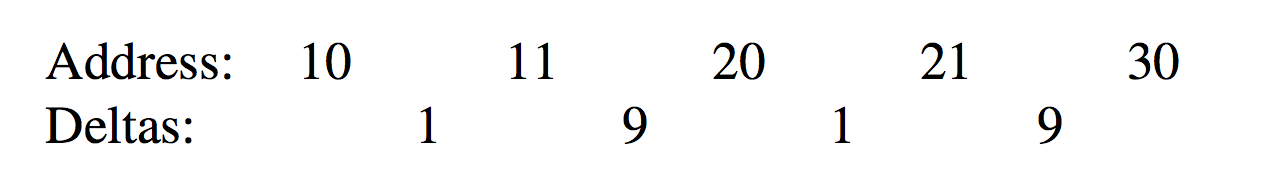
\includegraphics[width=0.35\textwidth]{Figures/DCExample}
  \caption{Example Delta Stream (Reprinted from \protect\cite{dcpt})}
  \label{fig:delta_stream}
\end{figure}

\subsection{Global History Buffer}

History based prefetchers need to store access patterns efficient data structure that enables quick access.
One such data structure is the Global History Buffer (GHB) \cite{ghb} which is shown in Fig.~\ref{fig:ghb}.
GHB is an $n$-entry First-In, First-Out (FIFO) queue implemented as a circular buffer.
It stores the $n$ most recent L1 cache misses in entries that contain the miss address and a link pointer.
The link pointer is used to chain entries together into time-ordered linked lists that holds the significant access patterns.
An Index Table (IT) is used to keep track of these lists.
It maps some key to the most recent element of a linked list.
The IT is based on a FIFO queue like GHB, but significantly smaller as each entry has to be evaluated for each cache miss to look up a matching key.
The key can be based on any cache miss information, and depending on it a wide variety of history based prefetch methods can be implemented.

\begin{figure}[!ht]
  \centering
      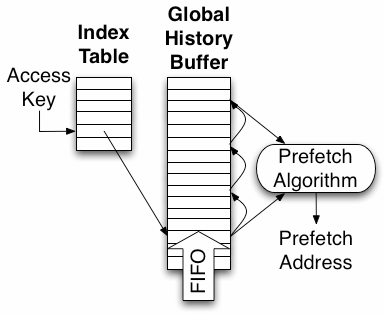
\includegraphics[width=0.3\textwidth]{Figures/ghb}
  \caption{Global History Buffer Structure (Reprinted from \protect{\cite{ghb}})}
  \label{fig:ghb}
\end{figure}

By keeping only recent data, it is not subject to any significant amount of stale data, and is better able to capture current access patterns.
Programs changing between several regular patterns may however not benefit from this, as one pattern might fill the whole buffer, causing information of the other to be lost.
In a comparison of different prefetch mechanisms by Péres et al.\cite{microlib}, one using GHB gave the best performance.

\section{Prefetcher Description}

A total of 5 different prefetchers have been implemented and tested: CZone Delta Correlation, Adaptive CZone Delta Correlation, Program Counter Delta Correlation, Adaptive Program Counter Correlation, and Delta Correlation Prediction Table. 
What they have in common is that they all implement Delta Correlation, and four use Global History Buffer (GHB). 
The following subsections will describe the differences between these:

\subsection{CZone Delta Correlation}

\begin{figure}[!ht]
  \centering
      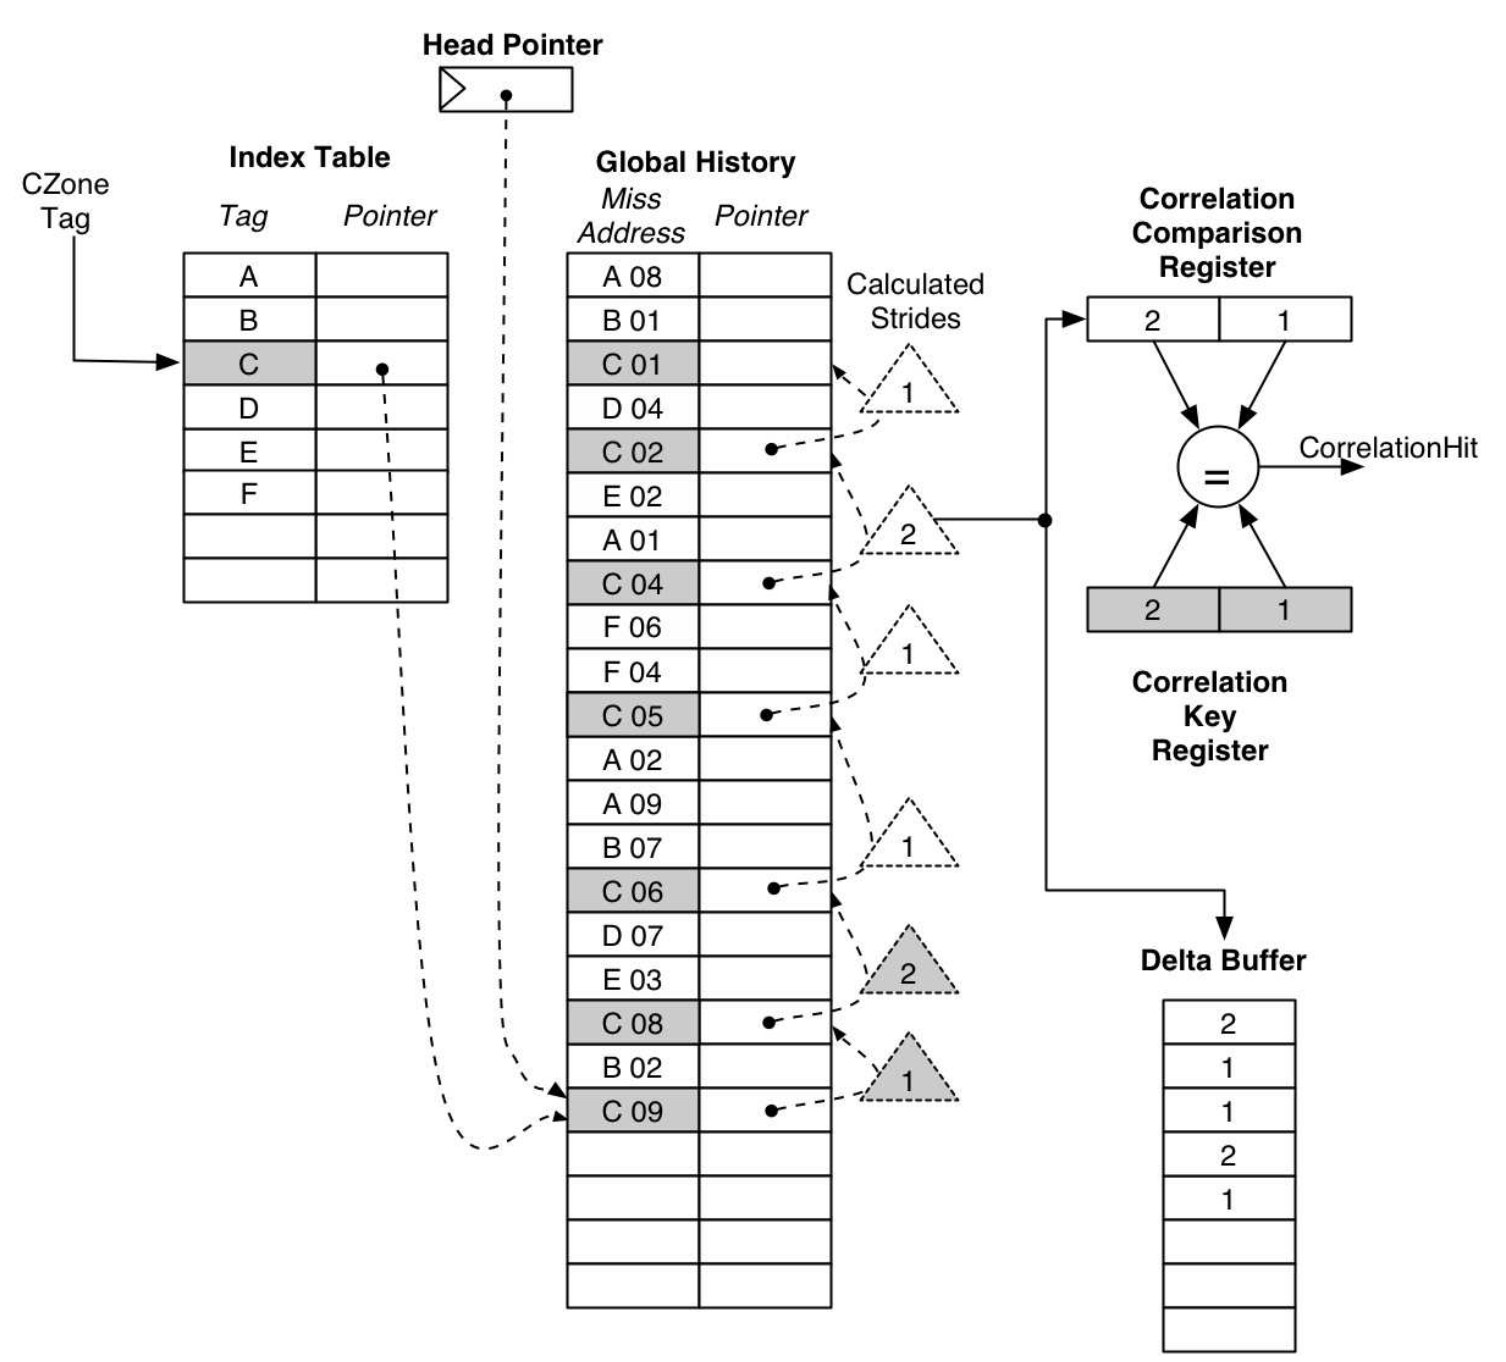
\includegraphics[width=0.5\textwidth]{Figures/CDC}
  \caption{CZone Delta Correlation (Reprinted from \protect\cite{acdc})}
  \label{fig:CDC}
\end{figure}

\todo{Rewrite this intro}
Fig.~\ref{fig:CDC} shows how CZone Delta Correlation works. 
The memory is divided into different concentration zones (CZones). 
The reason behind this is that memory load patterns from different areas of the memory may be different from each other, and the idea is to calculate correct prefetch based on the CZones of the load addresses.
The contents of the index table are based on the different CZones, and the pointer belonging to a CZone points to the latest address from that CZone that is stored in the GHB.
Fig.~\ref{fig:CDC} shows an example of a CZone Delta Correlation Prefetcher that implements GHB and Delta Correlation. 
Tag C from the index table points to address C09 from CZone C is the head, and is linked to C08,  which again is linked to C06, etc. 
The first two address deltas (1 and 2) from the linked list is added to the Correlation Key Register (2 and 1 in the example). 
The list is traversed, and the Correlation Comparison Register is continuously updated with the two latest deltas. 
When the correlation of the deltas of addresses C2-C4-C5 and C6-C8-C9  occurs, a delta buffer is filled with the deltas from the traversed list so far, and a prefetch based on the latest addresses and the deltas is issued.
Addresses C11, C12, C13, C15 and C16 will be calculated and prefetched.
 
\todo{ Write about head pointer?} \break

\subsection{Adaptive CZone Delta Correlation}
This is a more advanced version of the CZone Delta Correlation Prefetcher.
While the non-adaptive version prefetches a static number of data blocks, this one dynamically calculates how many data blocks to prefetch.
The prefetcher increases or decreases the number of blocks to be prefetched by 1, after evaluating the hit rate.
The hit rate is compared with the hit rate of the previous setting, and the prefetcher increases or decreases the number of blocks based on increased or decreased performance. 

\subsection{Program Counter Delta Correlation}
\todo{write something}
A load instruction in the PC may be used several times to load data from different addresses on the memory.
Addresses of a load instruction that misses is read from the PC and placed in the Index table, and it points to the latest missed data address connected to that specific instruction address. 

\subsection{Adaptive Program Counter Delta Correlation}
\todo{write something}
This is a more advanced version of the Program Counter Delta Prefetcher, that calculates how many blocks to load by comparing hit rate performance on the current load number with the previous load number.

\subsection{Delta Correlation Prediction Tables}

\todo{Describe how the final prefetcher works. I suggest adding a figure. Maybe briefly mention other attempts while if we have space?}


As can be seen, a row in the table contains fields for the PC, last address, last prefetch, deltas 1 to $ n $, and delta pointer.
PC stores the address to the load instruction, and works as index in the table.
The Last Address stores the missed address when there is a miss in the cache.
The delta fields stores the address difference, or the deltas, for each time this instruction is called.
Last prefetch contains the address of the last issued prefetch.
The Delta Pointer points to the head (first Delta field) in the row, since the delta fields are used as circular buffer.

\begin{figure}[h!]
  \centering
      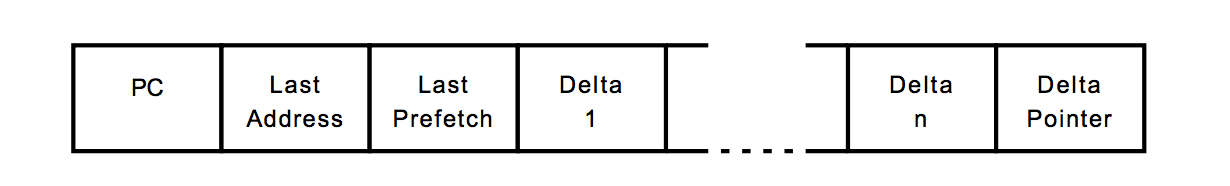
\includegraphics[width=0.5\textwidth]{Figures/DCTable}
  \caption{Delta Correlation Prediction Table}
  \label{fig:DCTable}
\end{figure}

\section{Methodology}

In order to measure prefetcher performance, a test bench had to be made.
Software implementations of the different prefetcher behaviors were implemented nd simulated in a simulation framework.

\subsection{Simulation Framework}

A modified version of M5, the open-source TCP/IP network simulator\cite{M5paper}, has been used to simulate a hierarchical memory environment for evaluation of the different prefetcher implementations.
The modified M5 simulator is supplied as course material.

The memory model simulated by the framework is based on the Alpha 21264 microprocessor, which is a superscalar processor capable of out-of-order execution through speculative execution and instruction reordering.

The modified M5 user guide documents the exact architecture details:

\begin{quote}
The L1 prefetcher is split in a 32kB instruction cache, and a 64kB data cache.
Each cache block is 64B.
The L2 cache size is 1MB, also with a cache block size of 64B.
The L2 prefetcher is notified on every access to the L2 cache, both hits and misses.
There is no prefetching for the L1 cache.

The memory bus runs at 400MHz, is 64 bits wide, and has a latency of 30ns.~\cite{m5userguide}
\end{quote}

To simulate a prefetcher with the modified M5 framework, the behavior must be implemented as an M5 prefetcher module in C++ and plugged into the system.
To emulate realistic conditions for a hardware prefetcher implementation, a hard memory usage limit of 8KB was imposed on the software prefetchers.
That means that a prefetcher may only allocate up to 8KB of memory to hold any eventual data structures.
No further restrictions were imposed.

\subsection{SPEC CPU2000}

To measure the performances of the different prefetchers, the prefetchers were simulated and observed during runs against a subset of the SPEC CPU2000 benchmark suite.~\cite{http://dl.acm.org/citation.cfm?id=621510}

The benchmarks measure several key performance indicators:

\subsubsection{Speedup}
Speedup is the total execution speedup gained by using a given prefetcher compared to having no prefetcher at all.

\subsubsection{IPC}
IPC, or Instructions Per Cycle, measures how many instructions are executed per clock cycle of the processor.
Since the simulated M5 architecture is superscalar, this number can be greater than 1.

\subsubsection{Accuracy}
Accuracy is a measure that shows how many prefetches were useful.

\subsubsection{Coverage}
Coverage is a measurement that answers the question of how many potential prefetch candidates were identified by the prefetcher.

\subsubsection{Identified}
Identified is a measure that shows how many prefetches have been issued to the cache controller by the prefetcher.

\subsubsection{Issued}
Issued is a measure that shows how many prefetches have been issued to the next memory hierarchy level by the cache controller.

\subsection{PFJudge}

PFJudge is a prefetcher judge system available through an online web interface.
It is used in this project to run the M5-based simulations.

\subsection{Development}

\todo{explain how the prefetchers were developed.}

\section{Results}

The results from the benchmark runs are shown in Fig. \ref{fig:results}.

\pgfplotstableread{
test_name        dcpt  apcdc cdc pcdc 
{ammp}           1.478 1.501 1   1
{applu}          1.088 1.077 1   1
{apsi}           1.037 1.010 1   1
{art110}         1.042 1.058 1   1
{art470}         1.042 1.058 1   1
{bzip2\_graphic} 1.145 1.067 1   1
{bzip2\_program} 1.035 1.040 1   1
{bzip2\_source}  1.004 1.006 1   1
{galgel}         1.040 1.082 1   1
{swim}           1.031 1.035 1   1
{twolf}          0.992 0.991 1   1
{wupwise}        1.226 1.238 1   1
}\speeduptable

\newcommand{\mgraph}[2]{
\begin{tikzpicture}[scale=0.5]
\begin{axis}[
  ybar, bar width=1pt,ymin=0,
  xmin=0.5,xmax=12.5, xtick=data,
  %axis y discontinuity=crunch,
  %ymin=0.75,
  xticklabels from table={#1}{test_name},
  xticklabel style={rotate=45,anchor=north east,inner sep=0mm},
  ylabel={\Large #2}, ylabel near ticks]
  \addplot table [x expr=\coordindex+1,y=dcpt] {#1};
  \addlegendentry{DCPT};
  \addplot table [x expr=\coordindex+1,y=apcdc] {#1};
  \addlegendentry{APCDC};
  \addplot table [x expr=\coordindex+1,y=cdc] {#1};
  \addlegendentry{CDC};
  \addplot table [x expr=\coordindex+1,y=pcdc] {#1};
  \addlegendentry{PCDC};
\end{axis}
\end{tikzpicture}
}

\newcommand{\mtable}[2]{
\centering
\resizebox{.81\columnwidth}{!}{
\pgfplotstabletypesetfile[
columns={test_name, dcpt, apcdc, cdc, pcdc},
every even row/.style={before row={\rowcolor{blue!15}}},
every head row/.style={
  before row={\toprule 
    \multirow{2}{*}{\bfseries Test Name} & \multicolumn{4}{c}{\bfseries #2}\\ \cmidrule{2-5}},
  after row=\midrule},
every last row/.style={after row=\bottomrule},
every row/.style={font=\tiny},
columns/test_name/.style={
  column name={},
  column type={l},
  string type},
columns/dcpt/.style={
  column name={DCPT},
  },
columns/apcdc/.style={
  column name={APCDC},
  },
columns/cdc/.style={
  column name={CDC},
  },
columns/pcdc/.style={
  column name={PCDC},
  },
    ] 
  {#1}
}
}


\pgfplotstableread{
test_name        dcpt  apcdc cdc pcdc 
{ammp}           1.478 1.501 1   1
{applu}          1.088 1.077 1   1
{apsi}           1.037 1.010 1   1
{art110}         1.042 1.058 1   1
{art470}         1.042 1.058 1   1
{bzip2\_graphic} 1.145 1.067 1   1
{bzip2\_program} 1.035 1.040 1   1
{bzip2\_source}  1.004 1.006 1   1
{galgel}         1.040 1.082 1   1
{swim}           1.031 1.035 1   1
{twolf}          0.992 0.991 1   1
{wupwise}        1.226 1.238 1   1
}\speeduptable
\pgfplotstableread{
test_name        dcpt  apcdc cdc pcdc 
{ammp}           0.122 0.124 1   1
{applu}          0.561 0.556 1   1
{apsi}           1.542 1.502 1   1
{art110}         0.127 0.129 1   1
{art470}         0.127 0.129 1   1
{bzip2\_graphic} 1.508 1.405 1   1
{bzip2\_program} 1.536 1.543 1   1
{bzip2\_source}  1.717 1.720 1   1
{galgel}         0.462 0.481 1   1
{swim}           0.705 0.708 1   1
{twolf}          0.421 0.420 1   1
{wupwise}        0.918 0.926 1   1
}\ipctable
\pgfplotstableread{
test_name        dcpt  apcdc cdc pcdc 
{ammp}           0.813 0.774 1   1
{applu}          0.636 0.525 1   1
{apsi}           0.403 0.355 1   1
{art110}         0.801 0.795 1   1
{art470}         0.801 0.795 1   1
{bzip2\_graphic} 0.896 0.788 1   1
{bzip2\_program} 0.807 0.574 1   1
{bzip2\_source}  0.782 0.702 1   1
{galgel}         0.655 0.739 1   1
{swim}           0.582 0.554 1   1
{twolf}          0.323 0.287 1   1
{wupwise}        0.667 0.667 1   1
}\accuracytable
\pgfplotstableread{
test_name        dcpt  apcdc cdc pcdc 
{ammp}           0.702 0.698 1   1
{applu}          0.332 0.336 1   1
{apsi}           0.173 0.028 1   1
{art110}         0.170 0.201 1   1
{art470}         0.170 0.201 1   1
{bzip2\_graphic} 0.755 0.577 1   1
{bzip2\_program} 0.537 0.229 1   1
{bzip2\_source}  0.625 0.459 1   1
{galgel}         0.425 0.924 1   1
{swim}           0.417 0.413 1   1
{twolf}          0.039 0.049 1   1
{wupwise}        0.667 0.651 1   1
}\coveragetable
\pgfplotstableread{
test_name        dcpt     apcdc    cdc pcdc 
{ammp}           13341801 19803635 1   1
{applu}          3243298  5414227  1   1
{apsi}           101119   16347    1   1
{art110}         14370198 54897828 1   1
{art470}         14370198 54897828 1   1
{bzip2\_graphic} 87717    72885    1   1
{bzip2\_program} 39751    23534    1   1
{bzip2\_source}  28729    23115    1   1
{galgel}         344166   781365   1   1
{swim}           2333012  4918637  1   1
{twolf}          156782   190970   1   1
{wupwise}        691877   551276   1   1
}\identifiedtable
\pgfplotstableread{
test_name        dcpt     apcdc     cdc pcdc 
{ammp}           12018716 112550456 1   1
{applu}          1160488  11423496  1   1
{apsi}           51421    19410     1   1
{art110}         2908765  13478208  1   1
{art470}         2908765  13478208  1   1
{bzip2\_graphic} 78988    168654    1   1
{bzip2\_program} 36835    122088    1   1
{bzip2\_source}  26851    122016    1   1
{galgel}         212199   1408948   1   1
{swim}           1622021  11688313  1   1
{twolf}          122898   1174298   1   1
{wupwise}        433846   1423433   1   1
}\issuedtable


\clearpage
\begin{figure*}[H]
\mgraph{\speeduptable}{Speedup}
\mgraph{\ipctable}{IPC}
\mgraph{\accuracytable}{Accuracy}
\mgraph{\coveragetable}{Coverage}
\mgraph{\identifiedtable}{Identified}
\mgraph{\issuedtable}{Issued}
\end{figure*}
\begin{figure*}[H]
\mtable{\speeduptable}{Speedup}
\mtable{\ipctable}{IPC}
\mtable{\accuracytable}{Accuracy}
\mtable{\coveragetable}{Coverage}
\mtable{\identifiedtable}{Identified}
\mtable{\issuedtable}{Issued}
\end{figure*}
\clearpage


\section{Discussion}

\todo{ Not exactly sure, just say it works better? Compare with other prefetcher IF we chose to describe them. }
All of the explored prefetching techniques resulted in improved performance in the tests, compared to no prefetching.
There are still differences, and none of the prefetching techniques is superior to the others in every test.
Overall the DCPT is scoring best on the test with APCDC on a close second.
Which of them would be best suited for a real life appliction, largely depend on the characteristics of the application.

\pgfplotstableread{
test_name  dcpt   apcdc pcdc  cdc   no_prefetcher
{}         1.0841 1.083 1.071 0.989 1.0
}\averagespeeduptable

\newcommand{\ngraph}[2]{
\begin{tikzpicture}[scale=0.5]
\begin{axis}[
  ybar, bar width=15pt,ymin=0,
  xmin=0.1,xmax=4, xtick=data,
  axis y discontinuity=crunch,
  ymin=0.9,
  xticklabels from table={#1}{test_name},
  xticklabel style={rotate=45,anchor=north east,inner sep=0mm},
  ylabel={\Large #2}, ylabel near ticks]
  \addplot table [x expr=\coordindex+1,y=dcpt] {#1};
  \addlegendentry{DCPT};
  \addplot table [x expr=\coordindex+1,y=apcdc] {#1};
  \addlegendentry{APCDC};
  \addplot table [x expr=\coordindex+1,y=cdc] {#1};
  \addlegendentry{CDC};
  \addplot table [x expr=\coordindex+1,y=pcdc] {#1};
  \addlegendentry{PCDC};
  \addplot table [x expr=\coordindex+1,y=no_prefetcher] {#1};
  \addlegendentry{No Prefetcher};
\end{axis}
\end{tikzpicture}
}
\begin{figure}[ht]
\centering
\ngraph{\averagespeeduptable}{Average speedup}
\caption{Average speedup}
\label{fig:speedup}
\end{figure}

% dcpc Blast #1 http://dm-ark.idi.ntnu.no/pf/184/details/
% apcdc APCDC#2 http://dm-ark.idi.ntnu.no/pf/166/details/
% cdc cdc-1-16 http://dm-ark.idi.ntnu.no/pf/1442/details/
% pcdc pcdc-2 http://dm-ark.idi.ntnu.no/pf/1447/details/


\section{Conclusion}

\todo{ Mention what could have been done better or different? Future ideas? }

\bibliography{bibliography}
\bibliographystyle{plain}
\nocite{*}

\begin{IEEEbiography}[{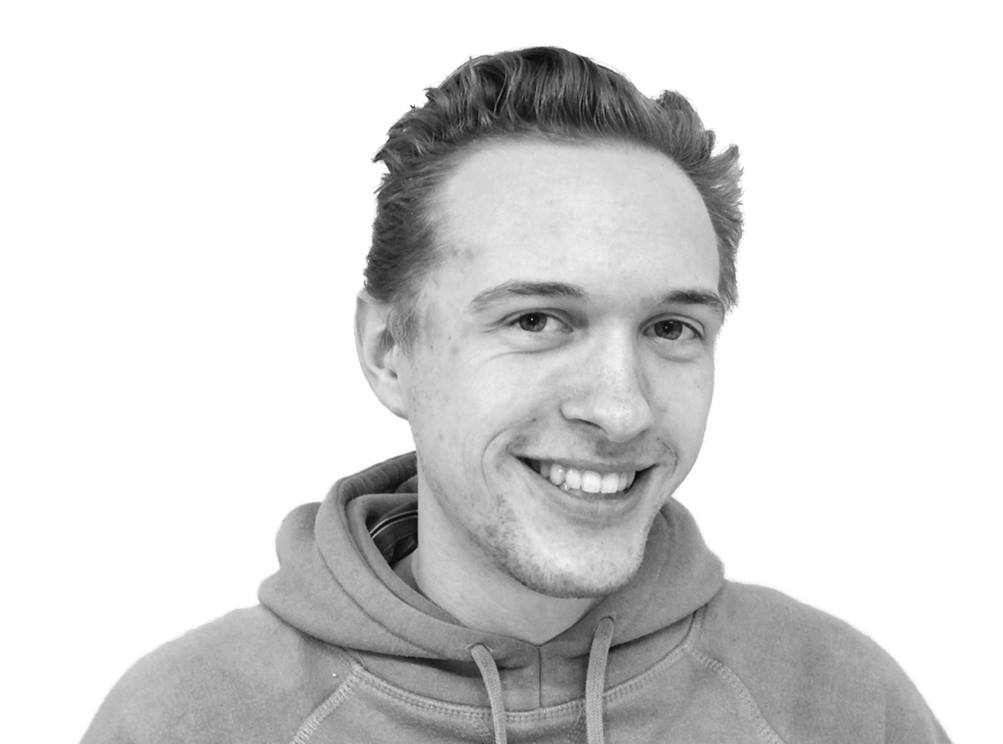
\includegraphics[width=1in,height=1.25in,clip,keepaspectratio]{Figures/farstad.jpg}}]{Sigve Sebastian Farstad}
    was born in Trondheim, Norway, in 1990.
    He is currently working towards an M.S. degree in computer science from the Norwegian University of Science and Technology, Trondheim, expecting to graduate in 2015.

    In 2009 he served as a civilian guardian of the Norwegian People, and he has since then worked as, amongst other things, a Software Consultant, a Technical Innovator in the mobile banking sector, a Professional Translator, and is currently working as one of the technical Co-Founders of feat.fm.

    Mr. Farstad was, together with other team members of the demo crew Ninjadev, the winner of the Web Demo Compo at Solskogen 2012.
\end{IEEEbiography}

\begin{IEEEbiography}[{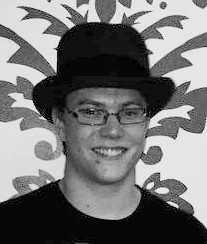
\includegraphics[width=1in,height=1.25in,clip,keepaspectratio]{Figures/holmgren.jpg}}]{Rune Holmgren}
    was born in Harstad, Norway, in 1991.
    He is currently working towards an M.S. degree in computer science from the Norwegian University of Science and Technology, Trondheim, expecting to graduate in 2015.

    He has worked as a Dairy Product Quality Assurance Intern, a Teaching Assistant for and most recently held the position of Summer Intern at Connome.

    Mr. Holmgren was recipient of the award Friidrettens Venners Kretspris in 2010.
\end{IEEEbiography}

\begin{IEEEbiography}[{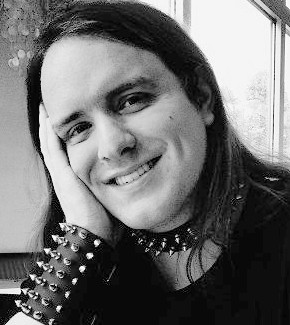
\includegraphics[width=1in,height=1.25in,clip,keepaspectratio]{Figures/langland.jpg}}]{Torbjørn Langland}
    was born in Trondheim, Norway, in 1987.
    He is currently working towards an M.S. degree in computer science from the Norwegian University of Science and Technology, Trondheim, expecting to graduate in 2015.

    He was worked as a Temporary Store Clerk and until recently held the title of Software Engineer at Comsol.

    Mr Langland is exceptionally good at playing Mario Kart 64.
\end{IEEEbiography}

\begin{IEEEbiography}[{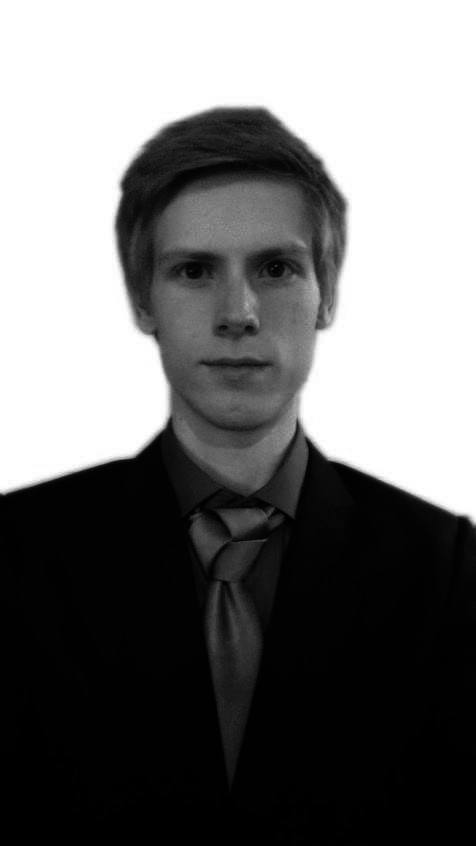
\includegraphics[width=1in,height=1.25in,clip,keepaspectratio]{Figures/lundal.jpg}}]{Per Thomas Lundal}
    was born in Trondheim, Norway, in 1991.
    He is currently working towards an M.S. degree in computer science from the Norwegian University of Science and Technology, Trondheim, expecting to graduate in 2015.

    He has since 2006 worked as a Sales Representative at Biltema.
    He has also worked as a Teaching Assistant for the course Programming Languages at NTNU.

    Mr. Lundal was the recipient of the Champions' Award and the Programming Award at the First Lego League, Trondheim.
\end{IEEEbiography}

\end{document}
